\documentclass[tikz,dvisvgm]{standalone}

\usepackage{cmbright}
\usepackage{amsmath} % for aligned
\usepackage{listofitems} % for \readlist to create arrays
\usetikzlibrary{arrows.meta} % for arrow size
\usepackage[outline]{contour} % glow around text
\contourlength{1.4pt}

% COLORS
\usepackage{xcolor}
\colorlet{myred}{red!80!black}
\colorlet{myblue}{blue!80!black}
\colorlet{mygreen}{green!60!black}
\colorlet{myorange}{orange!70!red!60!black}
\colorlet{mydarkred}{red!30!black}
\colorlet{mydarkblue}{blue!40!black}
\colorlet{mydarkgreen}{green!30!black}

% STYLES
\tikzset{
  >=latex, % for default LaTeX arrow head
  node/.style={thick,circle,draw=myblue,minimum size=22,inner sep=0.5,outer sep=0.6},
  node in/.style={node,green!20!black,draw=mygreen!30!black,fill=mygreen!25},
  node hidden/.style={node,blue!20!black,draw=myblue!30!black,fill=myblue!20},
  node convol/.style={node,orange!20!black,draw=myorange!30!black,fill=myorange!20},
  node out/.style={node,red!20!black,draw=myred!30!black,fill=myred!20},
  connect/.style={thick,mydarkblue}, %,line cap=round
  connect arrow/.style={-{Latex[length=4,width=3.5]},thick,mydarkblue,shorten <=0.5,shorten >=1},
  node 1/.style={node in}, % node styles, numbered for easy mapping with \nstyle
  node 2/.style={node hidden},
  node 3/.style={node out}
}
\def\nstyle{int(\lay<\Nnodlen?min(2,\lay):3)} % map layer number onto 1, 2, or 3

\begin{document}

% NEURAL NETWORK activation
% https://www.youtube.com/watch?v=aircAruvnKk&list=PLZHQObOWTQDNU6R1_67000Dx_ZCJB-3pi&index=1
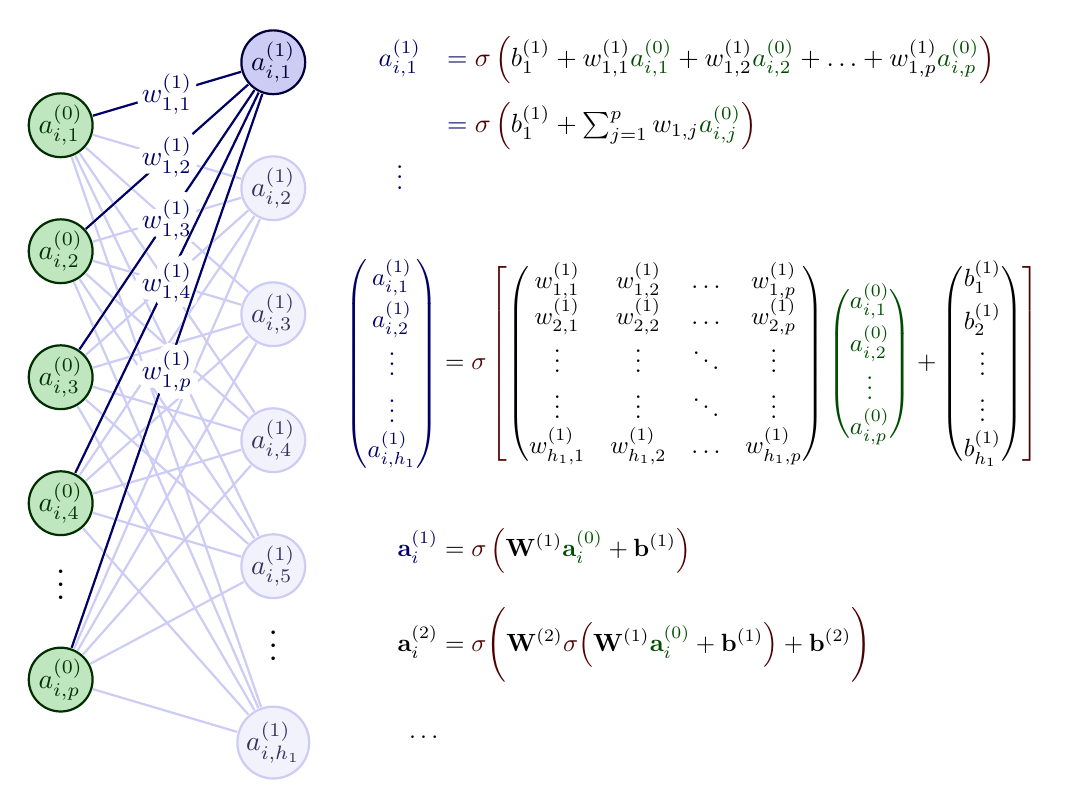
\begin{tikzpicture}[x=2.7cm,y=1.6cm]
  \message{^^JNeural network activation}
  \def\NI{5} % number of nodes in input layers
  \def\NO{6} % number of nodes in output layers
  \def\yshift{0.4} % shift last node for dots
  \contourlength{1mm};
  
  % INPUT LAYER
  \foreach \i [evaluate={\c=int(\i==\NI); \y=\NI/2-\i-\c*\yshift; \index=(\i<\NI?int(\i):"p");}]
              in {1,...,\NI}{ % loop over nodes
    \node[node in,outer sep=0.6] (NI-\i) at (0,\y) {$a_{i,\index}^{(0)}$};
  }
  
  % OUTPUT LAYER
  \foreach \i [evaluate={\c=int(\i==\NO); \y=\NO/2-\i-\c*\yshift; \index=(\i<\NO?int(\i):"h_1");}]
    in {\NO,...,1}{ % loop over nodes
    \ifnum\i=1 % high-lighted node
      \node[node hidden]
        (NO-\i) at (1,\y) {$a_{i,\index}^{(1)}$};
      \foreach \j [evaluate={\index=(\j<\NI?int(\j):"p");}] in {1,...,\NI}{ % loop over nodes in previous layer
        \draw[connect,white,line width=1.2] (NI-\j) -- (NO-\i);
        \draw[connect] (NI-\j) -- (NO-\i)
          node[pos=0.50] {\contour{white}{$w^{(1)}_{1,\index}$}};
      }
    \else % other light-colored nodes
      \node[node,blue!20!black!80,draw=myblue!20,fill=myblue!5]
        (NO-\i) at (1,\y) {$a_{i,\index}^{(1)}$};
      \foreach \j in {1,...,\NI}{ % loop over nodes in previous layer
        %\draw[connect,white,line width=1.2] (NI-\j) -- (NO-\i);
        \draw[connect,myblue!20] (NI-\j) -- (NO-\i);
      }
    \fi
  }
  
  % DOTS
  \path (NI-\NI) --++ (0,1+\yshift) node[midway,scale=1.2] {$\vdots$};
  \path (NO-\NO) --++ (0,1+\yshift) node[midway,scale=1.2] {$\vdots$};
  
  % EQUATIONS
  \def\agr#1{{\color{mydarkgreen}a_{i,#1}^{(0)}}} % green a_i^j
  \node[below=20,right=30,mydarkblue,scale=0.95] at (NO-1)
    {$\begin{array}{cl} %\underset{\text{bias}}{b_1}
      {\color{mydarkblue}a_{i,1}^{(1)}} &= \color{mydarkred}\sigma\left( \color{black}
            b_1^{(1)} + w^{(1)}_{1,1}\agr{1} + w^{(1)}_{1,2}\agr{2} + \ldots + w^{(1)}_{1,p}\agr{p}
          \color{mydarkred}\right)\\[1em]
       &= \color{mydarkred}\sigma\left( \color{black}
            b_1^{(1)} + \sum_{j=1}^{p} w_{1,j}\agr{j}
           \color{mydarkred}\right)\\
           \vdots
     \end{array}$};
  \node[right,scale=0.9] at (1.3,-1.5)
    {$\begin{aligned}
      {\color{mydarkblue}
      \begin{pmatrix}
        a_{i,1}^{(1)} \\[0.3em]
        a_{i,2}^{(1)} \\
        \vdots \\
        \vdots \\
        a_{i,h_1}^{(1)}
      \end{pmatrix}}
      &=
      \color{mydarkred}\sigma\left[ \color{black}
      \begin{pmatrix}
        w^{(1)}_{1,1} & w^{(1)}_{1,2} & \ldots & w^{(1)}_{1,p} \\
        w^{(1)}_{2,1} & w^{(1)}_{2,2} & \ldots & w^{(1)}_{2,p} \\
        \vdots  & \vdots  & \ddots & \vdots  \\
        \vdots  & \vdots  &  \ddots  & \vdots  \\
        w^{(1)}_{h_1,1} & w^{(1)}_{h_1,2} & \ldots & w^{(1)}_{h_1,p}
      \end{pmatrix}
      {\color{mydarkgreen}
      \begin{pmatrix}
        a_{i,1}^{(0)} \\[0.3em]
        a_{i,2}^{(0)} \\
        \vdots \\
        a_{i,p}^{(0)}
      \end{pmatrix}}
      +
      \begin{pmatrix}
        b_{1}^{(1)} \\[0.3em]
        b_{2}^{(1)} \\
        \vdots \\
        \vdots \\
        b_{h_1}^{(1)}
      \end{pmatrix}
      \color{mydarkred}\right]\\[2em]
      {\color{mydarkblue}\mathbf{a}_i^{(1)}} % vector (bold)
      &= \color{mydarkred}\sigma\left( \color{black}
           \mathbf{W}^{(1)} {\color{mydarkgreen}\mathbf{a}_i^{(0)}}+\mathbf{b}^{(1)}
         \color{mydarkred}\right)\\[1em]
      {\color{black}\mathbf{a}_i^{(2)}} % vector (bold)
      &= \color{mydarkred}\sigma\Bigg( \color{black}
           \mathbf{W}^{(2)}\color{mydarkred}\sigma\Big( \color{black}
           \mathbf{W}^{(1)} {\color{mydarkgreen}\mathbf{a}_i^{(0)}}+\mathbf{b}^{(1)}
         \color{mydarkred}\Big)
         \color{black}+\mathbf{b}^{(2)}
         \color{mydarkred}\Bigg)\\[1em]
         \hdots
    \end{aligned}$};
  
\end{tikzpicture}

\end{document}